\chapter{Exercises}








\section{Run a script}\label{exe:runascript}

Download this R-Script\footnote{\websmall\url{https://raw.githubusercontent.com/hubchev/R-Intro/master/scripts/SH-R-01.R} \textbf{Hint:} make a right-click and do \textit{save as}.} and try to run and use it in \Rstudio. This script shows some important features of \R and in particular, it installs the most important packages for you. In order to avoid problems in some examples later on in this course, please run this script.


\begin{rblock1}
	## ---------------------------
	## Script name: SH-R-01
	## Purpose of script: First script students should run
	## ---------------------------
	## Author: Dr. Stephan Huber
	## Date Created: 2020-09-30
	## Copyright (c) Stephan Huber, 2020
	## Email: Stephan.Huber(at)hs-fresenius.de
	## ---------------------------
	
	
	# Let us start with using R within RStudio
	# with a # you can write a comment in your script
	
	# with "Ctrl+Enter" you can execute a line of command, try it out:
	print("Hello, world!")
	
	# we use the book: "R for Dummies" in the course
	# when reading the book, always try to execute the code snippets by your own
	# For example, p. 3:
	# Simulate 1 million throws of two six‐sided dices:
	set.seed(42)
	throws <- 1e6
	dice <- replicate(2,
	sample(1:6, throws, replace = TRUE)
	)
	table(rowSums(dice))
	
	# with a "?" you get some help/information about the functions and operators used 
	?set.seed
	?assignOps
	?sample
	?hist
	?table
	
	# there are other ways to get help and learn within R
	help.start()
	example(hist)
	apropos("hist")
	vignette()
	vignette("ggwordcloud")
	
	# Performing multiple calculations with vectors
	24 + 7 + 11
	1 + 2 + 3 + 4 + 5
	14 / 2
	# but
	14 : 2 # this operator is called sequence
	3*2
	3      *       2
	# but > 3 x 2 does not work!
	x <- 1:5  # see assignment operator ?assignOps
	x
	x + 2
	x + 6:10
	x
	# alternatively:
	x2 <- x + 6:10
	x3 <- 6:10
	x4 <- x + x3
	
	# To construct a vector, type into the console:
	c(1, 2, 3, 4, 5)
	?c()
	b <- c(1, 2, 3, 4, 5)
	b
	
	# Packages are sort of R's brain so let's 
	# SEE WHAT PACKAGES ARE AROUND
	# https://www.r-pkg.org/
	# https://cran.r-project.org/web/views/
	# For example tidyvers and ggplot2 are powerfull packages to create data-visualizations, see:
	# https://www.r-graph-gallery.com/
	
	# LOAD PACKAGES 
	# There are a lot of packages pre-installed but not loaded, see here: 
	installed.packages()
	
	# A package can be installed using install.packages("<package name>"). 
	install.packages("dplyr")
	# A package can be removed using remove.packages("<package name>").
	remove.packages("dplyr")
	
	# I recommend "pacman" for managing add-on packages. It will
	# install packages, if needed, and then load the packages.
	install.packages("pacman")
	
	# Then load the package by using either of the following:
	require(pacman)  # Gives a confirmation message.
	library(pacman)  # No message.
	
	# Or, by using "pacman::p_load" you can use the p_load
	# function from pacman without actually loading pacman.
	# These are packages I load every time.
	pacman::p_load(pacman, dplyr, GGally, ggplot2, ggthemes, 
	ggvis, httr, lubridate, plotly, rio, rmarkdown, shiny, 
	stringr, tidyr) 
	
	
	# the package "datasets" contains some datasets 
	library(datasets)  # Load/unload base packages manually
	?datasets
	library(help = "datasets")
	
	# CLEAN UP #################################################
	
	# Clear packages
	p_unload(dplyr, tidyr, stringr) # Clear specific packages
	p_unload(all)  # Easier: clears all add-ons
	
	detach("package:datasets", unload = TRUE)  # For base
	
	# Clear console
	cat("\014")  # shortut for doing that is ctrl+L
\end{rblock1}

\section{How to load R built-in R data set mtcars and explore the data}\label{exe:mtcars}

Go to \url{https://t1p.de/R-mtcars} andsb-d write a script that contains the content of the page. Try to understand what is going on.
The pdf version of the file can be found on the following pages. 

%\section{tidyverse}\label{exe:tidyverse}	
%
%Check out the following script. Can you tell what is going on here?
%
%\begin{rblock1}
%	# The purpose of this script is to tell you all about scripts, 
%	# and to show you some of the cool things you can do with R.
%	#
%	# Here are a few things to note:
%	#
%	# 1. An R script is just a text file, and it ends with a .R file
%	#    extension. 
%	#
%	# 2. The main purpose of a script is to store a sequence of 
%	#    "commands", which are instructions to R that tell it what to do
%	# 
%	# 3. Any line that starts with a # is a "comment" and its main
%	#    purpose is to help out the humans! Your computer will ignore it
%	#    when it actually "executes" the script.
%	#
%	# 4. To make the script work, click on the "source" button in RStudio
%	#    (just above the top of this text!). 
%	#
%	# 5. When you click source, you'll see some output that appears in 
%	#    two places: the "console" (below) and in the "plots" panel (on
%	#    the right)
%	#
%	# 6. You may see some warning messages. That happens a lot - if you 
%	#    do, don't be too worried. That's pretty normal because R is 
%	#    usually very cautious :-) 
%	
%	install.packages("gapminder")
%	# packages
%	library(tidyverse)
%	library(gapminder)
%	
%	thisaredata <- gapminder
%	
%	# do some data manipulation and print to screen
%	gapminder %>% 
%	filter(country == "Australia") %>%
%	print()
%	
%	load(gapminder)
%	
%	# make a pretty picture 
%	pic <- gapminder %>% 
%	filter(continent == "Europe") %>%
%	ggplot(aes(x = year, y = lifeExp)) +
%	geom_line() + 
%	geom_point() + 
%	facet_wrap(~country)
%	
%	# plot the picture
%	plot(pic)
%	
%	# Some notes:
%	# 
%	# 1. Try to make sense of the table that has been printed to the console
%	# 2. Look at the graph. Think a bit about whether it could be improved.
%	# 3. Make an attempt to work out what the commands above (the "code") are
%	#    doing. Don't worry if you can't figure it out yet!
%\end{rblock1}


%\section{Regression}\label{exe:regression}
%
%Please consider the presentation on \textit{Regression Analysis} available on ILIAS. Please change the following script so that it runs on your PC. The necessary datasets are available on ILIAS.
%
%\begin{rblock1}
%	library(haven)
%	library(ggplot2)
%	library(sjPlot)
%	
%	rm(list = ls())
%	
%	# set working directory
%	setwd("~/Dropbox/hsf/courses_202/R/github/R-Intro")
%	
%	# load data from Stata format
%	classdata <- read_dta("~/Dropbox/hsf/courses_202/destat/classdata/classdata.dta")
%	
%	# or from csv data
%	classdata <- read.csv("~/Dropbox/hsf/courses_202/destat/classdata/classdata.csv")
%	
%	head(classdata)
%	
%	# first look at data
%	ggplot(classdata, aes(x=height, y=weight, shape = sex)) +
%	geom_point( aes(size = siblings)) 
%	
%	## baseline model
%	model  <- lm(weight ~ height + sex , data = classdata )
%	interw <- model$coefficients[1]+model$coefficients[3] 
%	interm <- model$coefficients[1] 
%	slope  <- model$coefficients[2]
%	
%	ggplot(classdata, aes(x=height, y=weight, shape = sex)) +
%	geom_point( aes(size = 2)) +
%	stat_smooth(formula = y ~ x,  method = "lm", se = FALSE, colour = "red", linetype = 1) +
%	geom_abline(slope = slope, intercept = interw, linetype = 2, size=1.5)+
%	geom_abline(slope = slope, intercept = interm, linetype = 2, size=1.5) +
%	geom_abline(slope = coef(model)[[2]], intercept = coef(model)[[1]]) 
%	
%	m1 <- lm(weight ~ height , data = classdata )
%	m2 <- lm(weight ~ height + sex , data = classdata )
%	m3 <- lm(weight ~ height + sex + height * sex , data = classdata )
%	m4 <- lm(weight ~ height + sex + height * sex + siblings , data = classdata )
%	m5 <- lm(weight ~ height + sex + height * sex , data = subset(classdata, siblings < 4 ))
%	
%	tab_model(m1, m2, m3, m4, m5,
%	p.style = "stars",
%	p.threshold = c(0.2, 0.1, 0.05),
%	show.ci = FALSE, 
%	show.se = FALSE) 
%	
%	plot(residuals(m4), fitted(m4))
%	plot(residuals(m4), classdata$siblings)
%\end{rblock1}
%




\includepdf[pages=-]{$HOME/Dropbox/hsf/22-ss/rcourse/rmd/mtcars_html.pdf}


\section{The pipe operator and others}\label{app:pipe}

\includepdf[pages=-]{$HOME/Dropbox/hsf/22-ss/rcourse/rmd/pipe-operator_html.pdf}


\section{Data transformation}

\boxx{
Please download and open the following R-script and try to answer the questions therein:

 \url{https://raw.githubusercontent.com/hubchev/courses/main/scr/data_transformation.R}
}

\begin{rblock1}
# ==============================================================================
# 0. 
# Set your working directory and clear the environment.

# ==============================================================================
# 1. 
# Download and read the most recent version of the lecture notes 
# (rcourse_book.pdf) from ILIAS.

# ==============================================================================
# 2. 
# Read: Wickham and Grolemund (2018, ch. "Workflow: basics"). 
# See: https://r4ds.had.co.nz/workflow-basics.html 

# ==============================================================================
# 3. 
# Answer the following questions:

# ===
# a) 
# Run the two following lines of code 
# (a.k.a. send it from the script to the console)
# Why does the second line of code not work? Look carefully! 
# This may seem like an exercise in pointlessness, but training your brain
# to notice even the tiniest difference will pay off when programming.)

my_variable <- 10
my_varıable

# ===
# b)
# Tweak each of the following R commands so that they run correctly:

library(tidyverse)

ggplot(dota = mpg) +
geom_point(mapping = aes(x = displ, y = hwy))

fliter(mpg, cyl = 8)
filter(diamond, carat > 3)

# Solutions:
ggplot(data = mpg) +
geom_point(mapping = aes(x = displ, y = hwy))

ggplot(data = mpg) + 
geom_point() +
aes(x = displ, y = hwy)

filter(diamonds, carat > 3)
filter(mpg, cyl == 8)
# ===
# c)
# Press Alt + Shift + K. What happens? How can you get to the same place using
# the menus?

# ==============================================================================
# 4. 
# Read Wickham and Grolemund (2018, ch. "Data transformation") 
# See: https://r4ds.had.co.nz/transform.html
# 
# Answer the following questions (Also see lecture notes excercise "Subsetting")
# 
# --- Solutions to these questions can be found here:
# https://raw.githubusercontent.com/hubchev/courses/main/scr/exe_subset.R
# !!! For your own benefit: try to come up with the solution yourself.  
# ===
# Load the following packages: tidyverse, dplyr, and tibble.
# ===
# Check to see if you have the mtcars dataset by entering the command mtcars.
# ===
# Save the mtcars dataset in an object named cars.
# ===
# What class is cars?
# ===
# How many observations (rows) and variables (columns) are in the 
# mtcars dataset?
# ===
# Rename mpg in cars to MPG. Use rename().
# ===
# Convert the column names of cars to all upper case. Use rename\_all, 
# and the toupper command.
# ===
# Convert the rownames of cars to a column called car using 
# rownames\_to\_column. 
# ===
# Subset the columns from cars that end in "p" and call it pvars 
# using ends\_with().
# ===
# Create a subset cars that only contains the columns: wt, qsec, and hp and 
# assign this object to carsSub.  (Use select().)
# ===
# What are the dimensions of carsSub? (Use dim().)
# ===# Convert the column names of carsSub to all upper case. Use rename\_all(), 
# and toupper() (or colnames()).
# ===
# Subset the rows of cars that get more than 20 miles per gallon (mpg) 
# of fuel efficiency. How many are there? (Use filter().)
# ===
# Subset the rows that get less than 16 miles per gallon (mpg) of fuel 
# efficiency and have more than 100 horsepower (hp). 
# How many are there? (Use filter() and the pipe operator.)
# ===
# Create a subset of the cars data that only contains the columns: wt, qsec, and
# hp for cars with 8 cylinders (cyl) and reassign this object to carsSub. 
# What are the dimensions of this dataset? Don't use the pipe operator.
# ===
# Create a subset of the cars data that only contains the columns: 
# wt, qsec, and hp for cars with 8 cylinders (cyl) and reassign 
# this object to carsSub2. Use the pipe operator.
# ===
# Re-order the rows of carsSub by weight (wt) in increasing order. 
# (Use arrange().)
# ===
# Create a new variable in carsSub called wt2, which is equal to $wt^2$, 
# using mutate() and piping \%>\%.

# ==============================================================================
# 5. 
# Read Wickham and Grolemund (2018, ch. "Data transformation") 
# See: https://r4ds.had.co.nz/transform.html
# Answer the question (1) of exercise 5.2.4 of Wickham and Grolemund (2018)
# See: 
# https://r4ds.had.co.nz/transform.html#exercises-8
# 
# Solutions can be found here:
# https://jrnold.github.io/r4ds-exercise-solutions/transform.html
# !!! For your own benefit: try to come up with the solution yourself. 
# ===
# Find all flights that
# ===
# Had an arrival delay of two or more hours
# ===
# Flew to Houston (IAH or HOU)
# ===
# Were operated by United, American, or Delta
# ===
# Departed in summer (July, August, and September)
# ===
# Arrived more than two hours late, but didn’t leave late
# ===
# Were delayed by at least an hour, but made up over 30 minutes in flight
# ===
# Departed between midnight and 6 am (inclusive)
\end{rblock1}

\section{Convergence}\label{sec:convergence}

The dataset convergence.dta, see  \url{https://github.com/hubchev/courses/blob/main/dta/convergence.dta}, contains the per capita GDP of 1960 (gdppc60) and the average growth rate of GDP per capita between 1960 and 1995 (growth) for different countries (country), as well as 3 dummy variables indicating the belonging of a country to the region Asia (asia), Western Europe (weurope) or Africa (africa). 

\begin{enumerate}[1)]
	\item Some countries are not assigned to a certain country group. Name the countries which are assign to be part of Western Europe, Africa or Asia.
	If you find countries that are members of the EU, assign them a '1' in the variable weurope.
	\item Create a table that shows the average GDP per capita for all available points in time. Group by Western European, Asian, African, and the remaining countries.
	\item Create the growth rate of GDP per capita from 1960 to 1995 and call it gdpgrowth. (Note: The log value X minus the log value X of the previous period is approximately equal to the growth rate).
	\item Calculate the unconditional convergence of all countries by constructing a graph in which a scatterplot shows the GDP per capita growth rate between 1960 and 1995 (gdpgrowth) on the y-axis and the 1960 GDP per capita (gdppc60) on the x-axis. Add to the same graph the estimated linear relationship. You do not need to label the graph further, just two things: title the graph `world' and label the individual observations with the country names.
%		Save the graph in Stata format with the label `world'.
%		(Note: If you cannot calculate gdpgrowth in Task 3, use the growth variable already in the dataset as an alternative).
	\item Create three graphs describing the same relationship for the sample of Western European, African and Asian countries. Title the graph accordingly with `weurope', `africa' and `asia'. 
	\item Combine the 4 graphs into one image. Discuss how an upward or downward sloping regression line can be interpreted.

	\item Estimate the relationships illustrated in the 4 graphs using the least squares method. Present the 4 estimation results in a table, indicating the significance level with stars. In addition, the Akaike information criterion, and the number of observations should be displayed in the table. Interpret the four estimation results regarding their significance. 
	\item Put the data set into the so-called \textit{long format} and calculate the GDP per capita growth rates for the available time points in the countries.
\end{enumerate}

\boxx{
	Please find solutions here: 
	\url{https://raw.githubusercontent.com/hubchev/courses/main/scr/convergence.R}
}


\section{Calories and weight}\label{exe:calories}
\boxx{
	Please find solutions here: 
	\url{https://raw.githubusercontent.com/hubchev/courses/main/scr/exe_calories.R}
}

\includepdf[pages=-]{$HOME/Dropbox/hsf/22-ss/dsda/tex/exe_calories.pdf}

\section{Forest and GDP}\label{exe:forest}
\boxx{
	Please find solutions here: 
	\url{https://raw.githubusercontent.com/hubchev/courses/main/scr/exe_forest_solution.R}
}

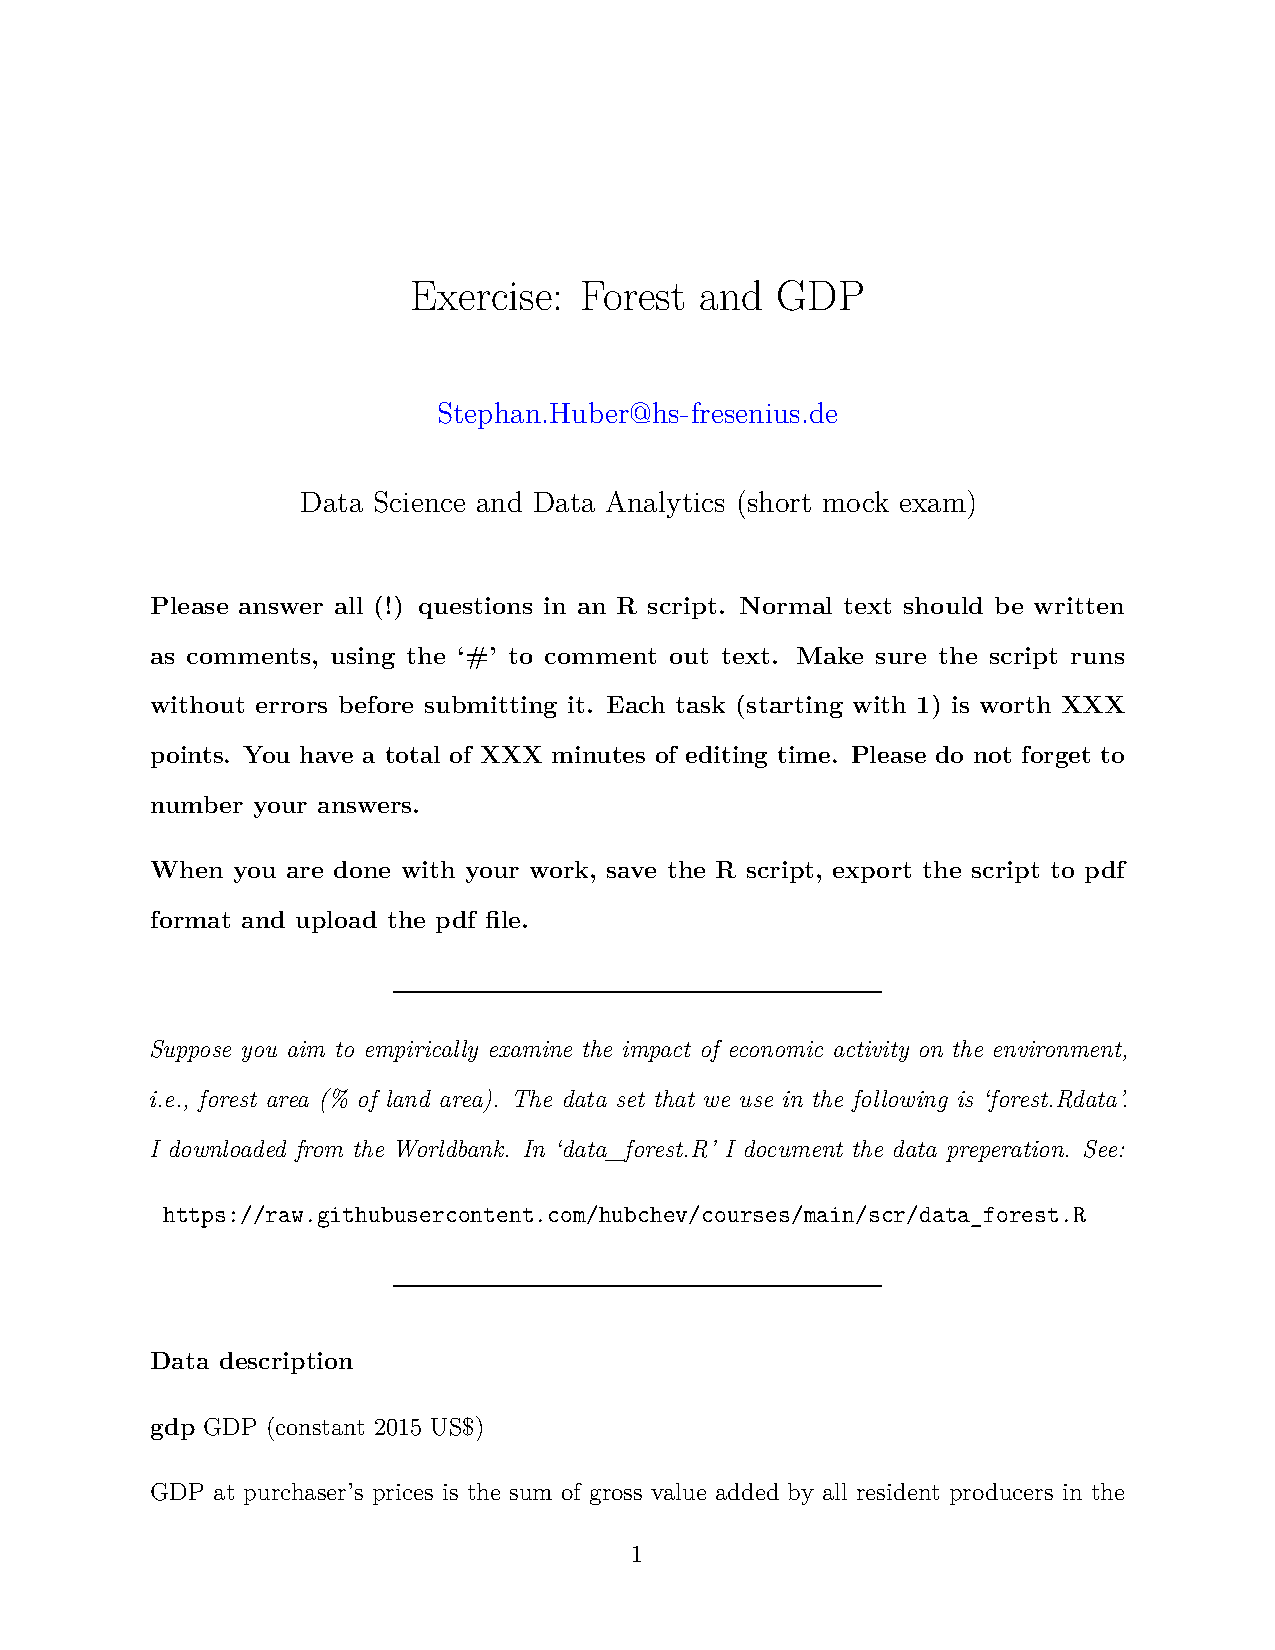
\includepdf[pages=-]{$HOME/Dropbox/hsf/github/courses/rmd/exe_forest.pdf}


\section{Unemployment and GDP in Germany and France}\label{exe:forest}
\boxx{
	Please find solutions here: 
	\url{https://raw.githubusercontent.com/hubchev/courses/main/scr/un_gdp_ger_fra.R}
}

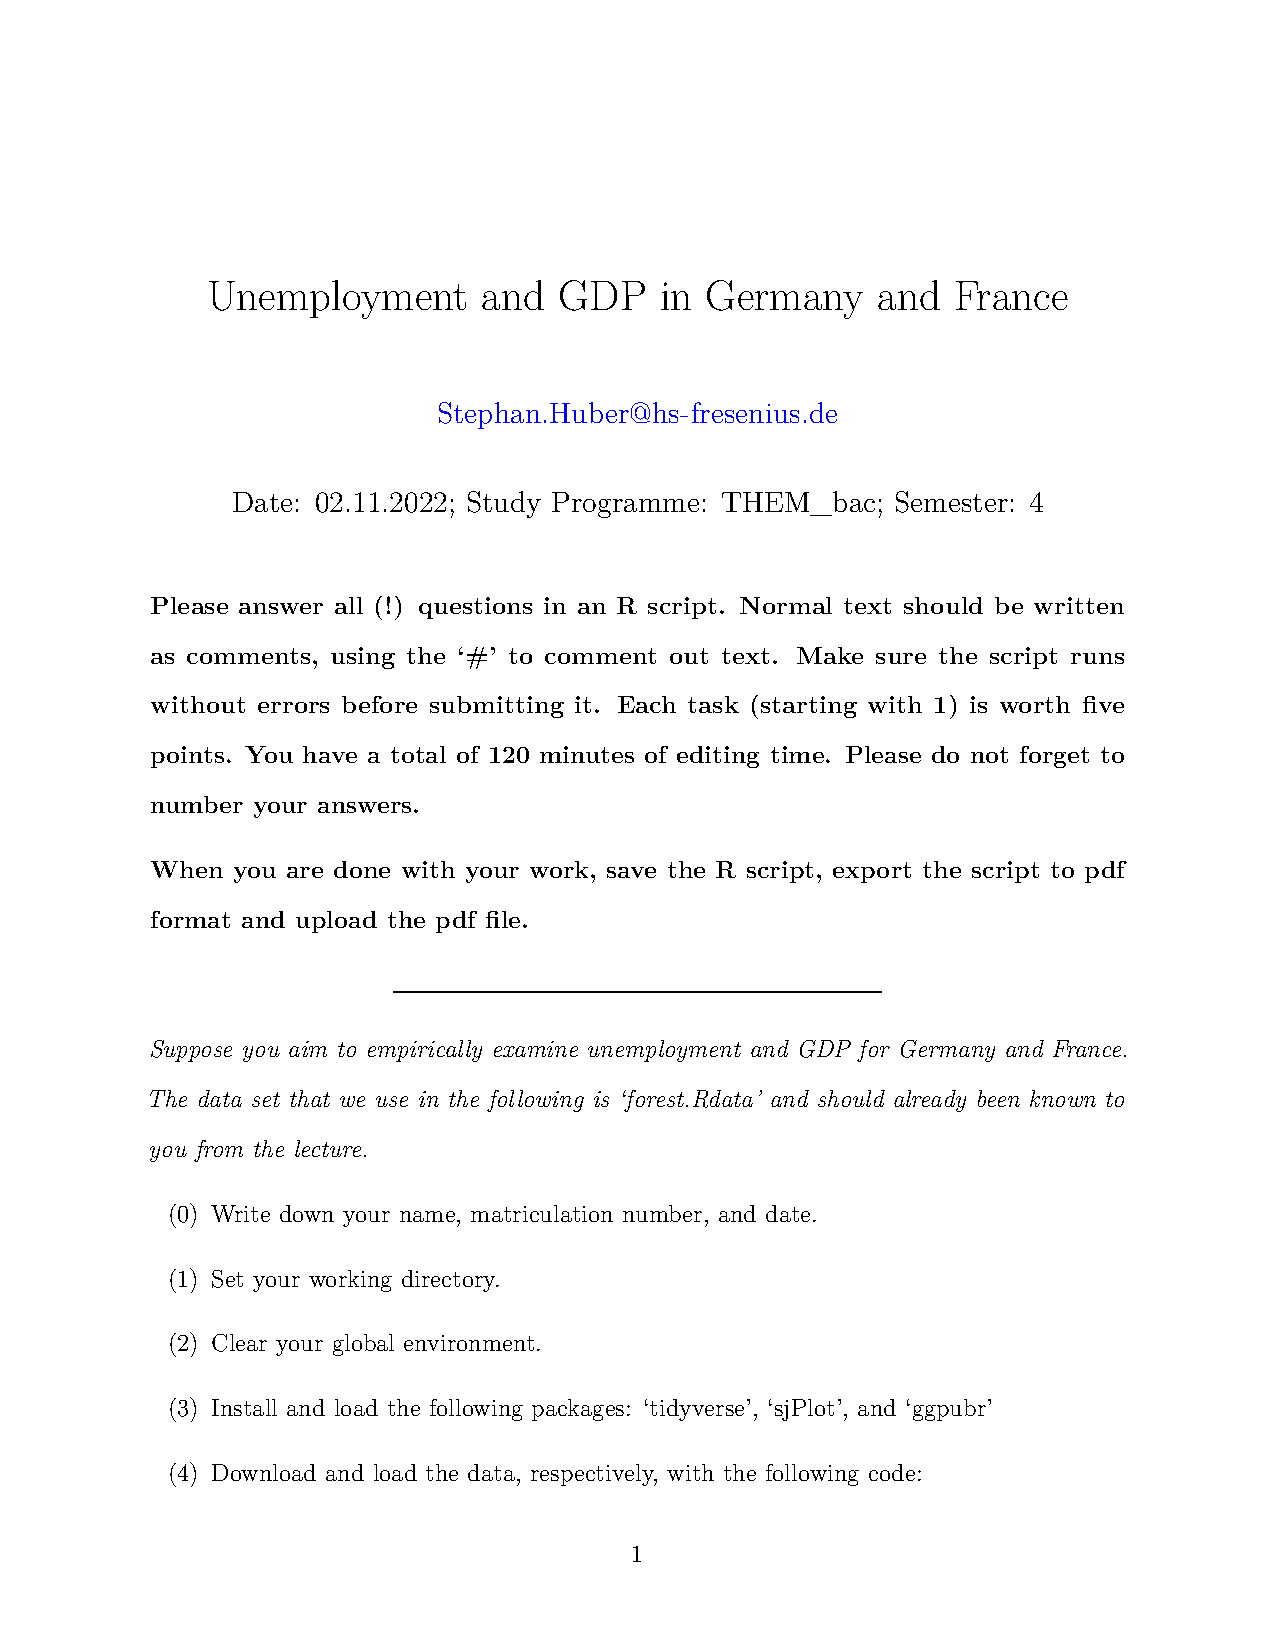
\includepdf[pages=-]{$HOME/Dropbox/hsf/github/courses/rmd/un_gdp_ger_fra.pdf}
